\documentclass[12pt,a4paper,oneside]{article}
\usepackage[colorlinks=true]{hyperref}
\usepackage[utf8]{inputenc}
\usepackage[czech]{babel}
\usepackage{graphicx}
\textwidth 16cm \textheight 25cm
\topmargin -1.3cm 
\oddsidemargin 0cm
\pagestyle{empty}
\begin{document}
\title{Softwarově definovaný přijímač SDRX01A}
\author{Jakub Kákona, kaklik@mlab.cz}
\maketitle

\begin{abstract}
\end{abstract}

\begin{figure} [htbp]
\begin{center}
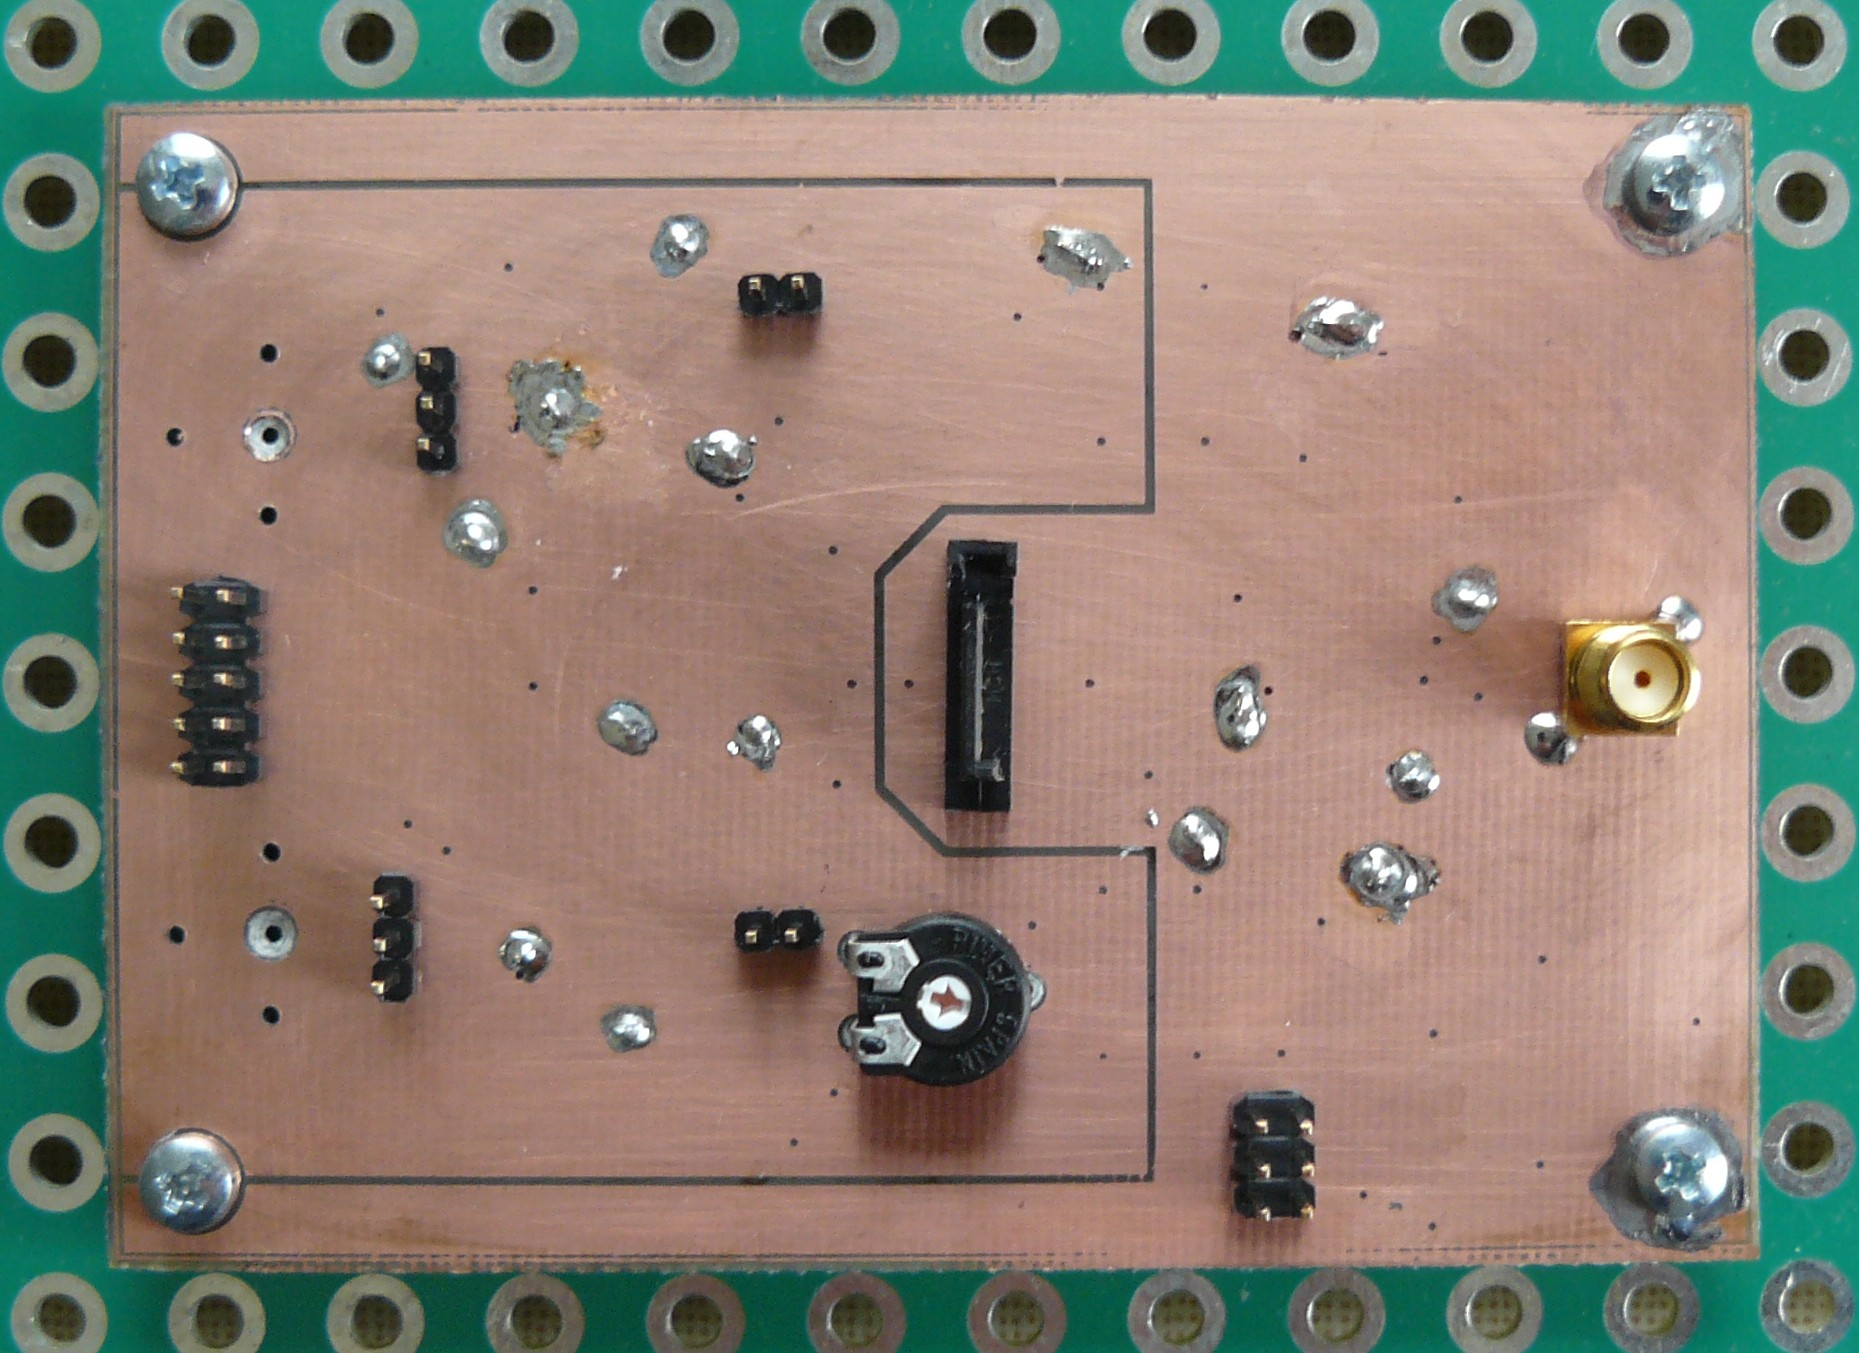
\includegraphics [width=80mm] {SDRX01A_Top_Big.JPG} 
\end{center}
\end{figure}

\tableofcontents

\section{Technické parametry}
\begin{table}[htbp]
\begin{center}
\begin{tabular}{|c|c|c|}
\hline
\multicolumn{1}{|c|}{Parametr} & \multicolumn{1}{|c|}{Hodnota} & \multicolumn{1}{|c|}{Poznámka} \\ \hline
Napájecí napětí analogové části & $\pm$10V &  100mA \\ \hline
Napájecí napětí digitální části & +5V &  300mA \\ \hline
Napájecí napětí LNA & do +20V &  max 500mA \\ \hline
Šumové číslo  & $<$ 30dB & \\ \hline
\end{tabular}
\end{center}
\end{table}

\newpage
\section{Popis konstrukce}

\subsection{Zapojení}
Zapojení přijímače vychází z původní konstrukce SDR přijímače DR2G \cite{DR2G}  který požívá starší součástky. Nyní má změněný hlavně obvod vstupu pro lokální oscilátor a umožňuje tak používat přijímač na vyšších kmitočtech, neboť nedělí vstupní frekvenci 4mi, jako původní konstrukce ale pouze 2mi. To mimo jiné znamená, že nejvyšší pracovní kmitočet již není limitován vstupní logikou, ale analogovými spínači a v menší míře i převodníky LVPECL-CMOS těsně před spínači. Použitá diferenciální LVPECL logika navíc také umožňuje podstatně snížit vyzařování. Dále byly vyměněny analogové spínače ve směšovači. Ty nyní spínají trochu rychleji, ale hlavně mají lepší izolační parametry, což umožňuje lepší odstup signálu od šumu.


Další nezbytnou saoučástí přijímače je lokální oscilátor, který se připojuje k přijímači pomocí krátkého SATA kabelu. Jako LO lze použít modul CLKGEN01 osazený 570ABB000107DG. SATA kabel je vhodné volit co nejkratší kvůli minimalizaci zemní smyčky a vyzařování. 

\subsection{Mechanická konstrukce}

Mechanická konstrukce je řešena na dvouvrstvé desce s rozměry kompatibilními se základovou deskou MLAB. Dvouvrstvá deska je zvolena hlavně kvůli kvalitnímu odstínění okolního rušení horní měděnou vrstvou. To umožňuje přijímače instalovat i velmi blízko sebe případně i nad sebe avšak všechny konektory  kromě NF audio výstupu předpokládají přivedení kabelu kolmo na rovinu desky. SMA konektor je možné osadit i úhlový s přivedením kabelu do boku, ale za cenu nepatrně vyššího útlumu úhlového konektoru. Při těsné montáži je potřeba počítat i s určitou teplotní stabilizací, neboť digitální část okolo spínaného směšovače má poměrně velký příkon a způsobuje zahřívání zhruba o 15$^\circ C$ nad okolní teplotu. 

\section{Výroba a testování}
Výrobu vlastní desky pro přijímač nemohu doporučit. Neboť domácí výroba je dvouvrstvého plošného spoje je náročná sama o sobě a tento motiv plošného spoje navíc obsahuje plošky pro komponenty s poměrně vysokou třídou přesnosti.

\subsubsection{Osazení}
Vlastní osazeni přijímače předpokládá zvládnutí SMT technologie. Nejkomplikovanější část je letování analogových spínačů u kterých je nutné dát pozor na přehřátí a je tedy vhodné použít více pastového tavidla.

\subsubsection{Nastavení}
Pokud je přijímač osazen bez chyb a zkratů, tak nastavení přijímače spočívá v opatrném připojení na napájecí napětí. (Symetrický napájecí zdroj musí být dostatečně kvalitní a vyhlazený, aby nedocházelo k průniku rušení do analogové části. Je též vhodné aby zdroj měl proudové omezení.) A nastavení shodných amplitud obou výstupních kanálů I a Q na stejnou úroveň pomocí trimru na horní straně desky. To lze udělat buď pomocí zvukové karty a minimalizace zrcadlových kmitočtů nějakého relativně silného AM vysílače a nebo přesněji pomoci dvoukanálového osciloskopu v libovolné části pásma. Lze použít i metodu, kdy pomocí Jumperů, které slouží na výběr zesílení odpojíme jeden kanál (ten ve větvi s trimrem) a v softwaru si označíme aktuální úroveň signálu z antény. Pak analogicky kanál odpojíme připojíme naopak ten původně odpojený. Pomocí trimru pak nastavíme stejnou hodnotu signálu. Tento způsob je velmi jednoduchý a lze ho použít i za chodu. Ale že je potřeba ještě zkontrolovat fázový posun, který by mezi kanály měl být $\pi / 2$. 

\section{Programové vybavení}

Základním programovým vybavením jsou všechny softwary využívající zvukovou kartu v komplexním režimu  pro vstup signálu. Tedy například programy jako Winrad či Spectrum Lab.

\begin{thebibliography}{99}
\bibitem{DR2G}{Původní konstrukce přijímače DR2G} 
\href{http://yu1lm.qrpradio.com/SMT SDR RX DR2G-YU1LM.pdf}{http://yu1lm.qrpradio.com/SMT SDR RX DR2G-YU1LM.pdf}

\end{thebibliography}
\end{document}